%%%%%%%%%%%%%%%%%%%%%%%%%%%%%%%%%%%%%%%%%%%%%%%%%%%%%%%%%%%%%%%%%%%%%%%%%%%%%%%%
\chapter{РАЗРАБОТКА АЛГОРИТМА ИЗВЛЕЧЕНИЯ КОНТРАКТОВ ИЗ ИСХОДНОГО КОДА}
\label{chapter:algoritm}
%%%%%%%%%%%%%%%%%%%%%%%%%%%%%%%%%%%%%%%%%%%%%%%%%%%%%%%%%%%%%%%%%%%%%%%%%%%%%%%%
В соответствии с поставленной задачей, необходимо разработать технологию автоматического извлечения контрактов функций из исходного кода программ. Технология состоит из трех основных элементов:
\begin{itemize}
\item анализ исходного кода программы и выявление предварительных версий контрактов;
\item хранение полученной информации;
\item получение окончательных версий контрактов для функций из извлеченной информации;
\end{itemize}

Этот раздел посвящен разработке перечисленных компонентов. В разделе изложены основные идеи, положенные в их основу. В разделе также рассмотрена модель представления кода, для которой разрабатывался алгоритм.

%%%%%%%%%%%%%%%%%%%%%%%%%%%%%%%%%%%%%%%%%%%%%%%%%%%%%%%%%%%%%%%%%%%%%%%%%%%%%%%%
\section{Общая схема алгоритма автоматического извлечения контрактов}
%%%%%%%%%%%%%%%%%%%%%%%%%%%%%%%%%%%%%%%%%%%%%%%%%%%%%%%%%%%%%%%%%%%%%%%%%%%%%%%%
Предлагаемая схема извлечения контрактов из исходного кода в общем виде может быть представлена следующим образом(см. рисунок \ref{image:generalScheme}). На схеме приведен алгоритм извлечения контрактов для одной функции.
\begin{figure}[h!]
\center{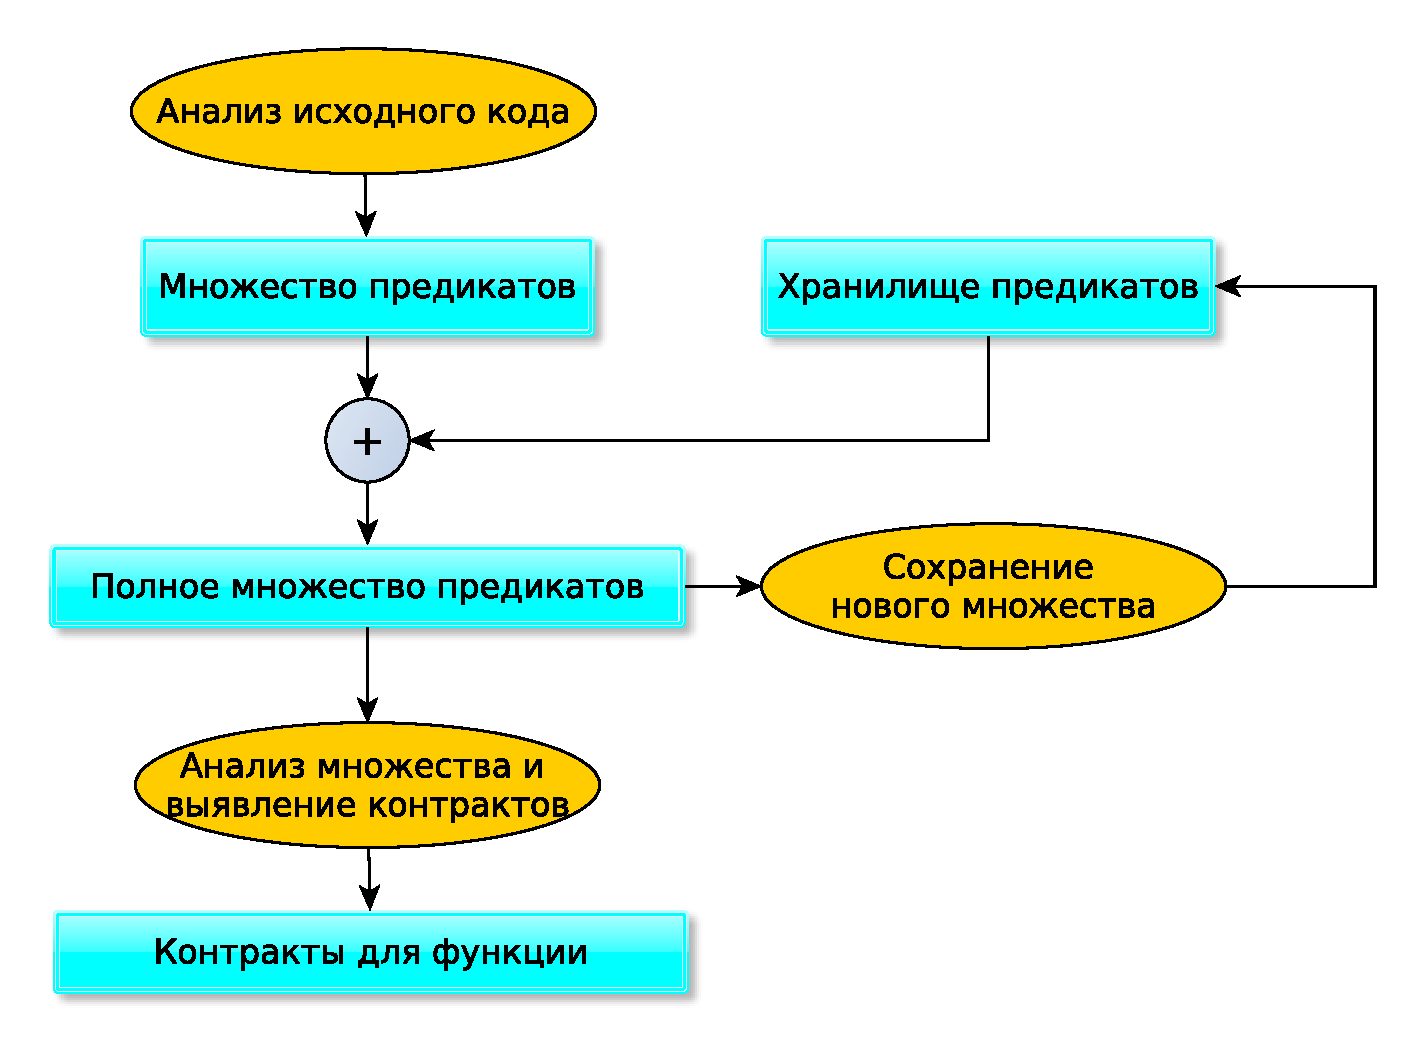
\includegraphics[width=\linewidth]{generalScheme}}
\caption{Общая схема технологии извлечения контрактов для функции из исходного кода}
\label{image:generalScheme}
\end{figure}

Алгоритм принимает на вход исходный код программы. На выходе --- сформированные контракты для функций, используемых в поданной программе. Для повышения эффективности работы алгоритма в нем так же используется хранилище предикатов. При выполнении анализа из него извлекается дополнительная информация о функции.

Главным показателем эффективности алгоритма является точность анализа, то есть вероятность извлечения некорректного контракта для функции должна быть минимальной. Остальные параметры (точность, эффективность) в данной работе считаются второстепенными.

Рассмотрим основные компоненты методики отдельно.

%%%%%%%%%%%%%%%%%%%%%%%%%%%%%%%%%%%%%%%%%%%%%%%%%%%%%%%%%%%%%%%%%%%%%%%%%%%%%%%%
\section{Модель представления кода исходной программы}
%%%%%%%%%%%%%%%%%%%%%%%%%%%%%%%%%%%%%%%%%%%%%%%%%%%%%%%%%%%%%%%%%%%%%%%%%%%%%%%%

%%%%%%%%%%%%%%%%%%%%%%%%%%%%%%%%%%%%%%%%%%%%%%%%%%%%%%%%%%%%%%%%%%%%%%%%%%%%%%%%
\subsection{Система LLVM}
%%%%%%%%%%%%%%%%%%%%%%%%%%%%%%%%%%%%%%%%%%%%%%%%%%%%%%%%%%%%%%%%%%%%%%%%%%%%%%%%
LLVM (Low Level Virtual Machine) --- универсальная система анализа, трансформации и оптимизации программ, реализующая виртуальную машину с RISC-подобными инструкциями\cite{llvm}. Центральным звеном LLVM является так называемое промежуточное представление (Intermediate Representation, IR), представляющее собой строго типизированный мета-ассемблер с бесконечным числом доступных для использования регистров.  Такая форма представления кода в LLVM (в виде IR) позволяет производить большое количество оптимизаций прямо над промежуточным представлением без необходимости учета особенностей исходного языка программирования, а строгая система типов делает код удобным для восприятия и позволяет производить преобразования, которые не представляется возможным выполнить при обычном трехадресном нетипизированном представлении кода.

Одной из самых важных частей LLVM является система проходов. Проходы (Passes) отвечают за трансформацию и оптимизацию промежуточного представления и объединяют результаты различных анализов для их использования в дальнейших преобразованиях.
\begin{figure}[h!]
\center{\includegraphics[width=\linewidth]{llvmIR}}
\caption{Пример представления функции в LLVM}
\label{image:llvmIR}
\end{figure}

Программы в LLVM представляются в виде набора отдельных модулей. Каждый модуль состоит из функций, глобальных переменных и дополнительных метаданных. Каждая функция, в свою очередь, состоит из базовых блоков. Каждый базовый блок имеет свою метку и состоит из последовательности инструкций, заканчивающейся инструкцией-терминатором, которая явно передает управление в другой блок или завершает выполнение текущей функции. Инструкция ret, завершающая выполнение функции, может быть только одна и всегда является самой последней инструкцией в функции. Пример представления программы в системе LLVM приведен на рисунке \ref{image:llvmIR}.
	
Переменные исходной программы в LLVM представляются в виде регистров (память на стеке) или в виде указателей на память (память на куче). Для регистров LLVM реализует статическое однократное присваивание (Static Single Assigment, SSA) --- форма представления кода, при которой любое значение присваивается только один раз. Любому регистру в LLVM можно присвоить значение только один раз --- при его объявлении. Для объединения потенциально различных значений одной и той же переменной исходной программы в SSA (то есть, и в LLVM) используются так называемые phi-функции, которые возвращают одно из значений в зависимости от того, какой блок передал управление текущему при выполнении программы.

%%%%%%%%%%%%%%%%%%%%%%%%%%%%%%%%%%%%%%%%%%%%%%%%%%%%%%%%%%%%%%%%%%%%%%%%%%%%%%%%
\subsection{Представление программ в системе <<Borealis>>}
%%%%%%%%%%%%%%%%%%%%%%%%%%%%%%%%%%%%%%%%%%%%%%%%%%%%%%%%%%%%%%%%%%%%%%%%%%%%%%%%
Система Borealis использует LLVM IR для компиляции, трансформации и анализа программ. Для упрощения взаимодействия различных компонентов системы Borealis добавляет еще один уровень промежуточного представления в виде predicate state API (PS API). Упрощенное описание PS в форме Бэкуса-Наура приведено на рисунке \ref{image:predicate-state-definition}.
	
Инструкции LLVM преобразуются в предикаты (predicate), которые выполняют различные операции над термами (term). Термы используются для представления констант, переменных, бинарных операций. Каждый терм так же может являться операндом другого терма или предиката. Предикаты соответствуют остальным инструкциям LLVM.
	
Предикаты в системе имеют различные типы. Всего определено 6 типов предикатов:
\begin{itemize}
\item State --- обычные предикаты, соответствующие инструкциям LLVM;
\item Path --- предикаты пути соответствуют условиям перехода в различные ветки развития программы;
\item Requires --- предикаты, использующиеся для выражения предусловий функций;
\item Ensures --- предикаты, использующиеся для выражения постусловий функций;
\item Assert --- предикаты, соответствующие assertion'ам в исходном коде;
\item Assume --- предикаты, позволяющие задавать утверждения, которые всегда верны.
\end{itemize}

\begin{figure}
	\begin{grammar}
	\scriptsize
	<PredicateState> ::= PredicateStateChain head:<PredicateState> tail:<PredicateState>
	\alt PredicateStateChoice choices:<ListOfPredicateStates>
	\alt BasicPredicateState data:<ListOfPredicates>

	<ListOfPredicateStates> ::= <PredicateState> <ListOfPredicateStates> | <empty>

	<Predicate> ::= AllocaPredicate lhv:<Term> numElems:<Term> origNumElems:<Term>
	\alt DefaultSwitchCasePredicate cond:<Term> cases:<ListOfTerms>
	\alt EqualityPredicate lhv:<Term> rhv:<Term>
	\alt GlobalsPredicate globals:<ListOfTerms>
	\alt InequalityPredicate lhv:<Term> rhv:<Term>
	\alt MallocPredicate lhv:<Term> numElems:<Term> origNumElems:<Term>
	\alt SeqDataPredicate base:<Term> data:<ListOfTerms>
	\alt SeqDataZeroPredicate base:<Term> size:UInt32
	\alt StorePredicate ptr:<Term> value:<Term>
	\alt WriteBoundPredicate ptr:<Term> boundValue:<Term>
	\alt WritePropertyPredicate propName:<Term> ptr:<Term> propValue:<Term>
	
	\tiny
	<Term> ::= ArgumentTerm idx:UInt32 kind:<ArgumentKind>
	\alt ArgumentCountTerm
	\alt AxiomTerm term:<Term> axiom:<Term>
	\alt BinaryTerm op:<BinaryOp> lhv:<Term> rhv:<Term>
	\alt BoundTerm term:<Term>
	\alt CastTerm term:<Term> signExtend:Bool
	\alt CmpTerm op:<CmpOp> lhv:<Term> rhv:<Term>
	\alt ConstTerm
	\alt FreeVarTerm
	\alt GepTerm base:<Term> shifts:<ListOfTerms> triviallyInbounds:Bool
	\alt LoadTerm ptr:<Term>
	\alt OpaqueBigIntConstantTerm value:String
	\alt OpaqueBoolConstantTerm value:Bool
	\alt OpaqueBuiltinTerm vname:String
	\alt OpaqueCallTerm func:<Term> args:<ListOfTerms>
	\alt OpaqueFloatingConstantTerm value:Double
	\alt OpaqueIndexingTerm value:<Term> index:<Term>
	\alt OpaqueIntConstantTerm value:SInt64
	\alt OpaqueInvalidPtrTerm
	\alt OpaqueMemberAccessTerm value:<Term> property:String indirect:Bool
	\alt OpaqueNamedConstantTerm vname:String
	\alt OpaqueNullPtrTerm 
	\alt OpaqueStringConstantTerm value:String
	\alt OpaqueUndefTerm 
	\alt OpaqueVarTerm vname:String
	\alt ReadPropertyTerm propName:<Term> ptr:<Term>
	\alt ReturnPtrTerm funcName:String
	\alt ReturnValueTerm funcName:String
	\alt SignTerm value:<Term>
	\alt TernaryTerm cond:<Term> tru:<Term> fls:<Term>
	\alt UnaryTerm op:<UnaryOp> value:<Term>
	\alt ValueTerm global:Bool
	\alt VarArgumentTerm index:UInt32

	<ListOfTerms> ::= <Term> <ListOfTerms> | <empty>

	<ArgumentKind> ::= ANY | STRING

	<BinaryOp> ::= ...
	<UnaryOp> ::= ...
	<CmpOp> ::= ...
	\end{grammar}
	
\caption{Определение PS в форме Бэкуса-Наура}
\label{image:predicate-state-definition}
\end{figure}

Predicate state ставится в соответствие каждой функции программы. При этом, как показано на рисунке \ref{image:predicate-state-definition}, PS может состоять как из предикатов, так и из других predicate state'ов. Вложенные PS обычно соответствуют базовым блокам LLVM IR. Predicate state имеет три вида:
\begin{enumerate}
\item Basic PS --- PS, соответствующий базовым блокам LLVM.
\item Choice PS --- PS, который позволяет реализовывать ветвления. Каждой веткой choice PS выбора может быть любой другой PS. Это позволяет представлять операторы множественного выбора и множественные ветвления. При этом стоит отметить, что в начале каждого PS, соответствующего какой-либо ветке, будет стоять path predicate, определяющий условия входа в эту ветку.
\item Chain PS --- PS, позволяющий объединить несколько PS в единую последовательность. Используется для соединения Basic PS и Choice PS в единую структуру.
\end{enumerate}

Предлагаемый подход автоматического извлечения контрактов будет описываться в терминах приведенной модели кода. Перейдем к более подробному рассмотрению этапов предлагаемой методологии.

%%%%%%%%%%%%%%%%%%%%%%%%%%%%%%%%%%%%%%%%%%%%%%%%%%%%%%%%%%%%%%%%%%%%%%%%%%%%%%%%
\section{Анализ исходного кода программы для извлечения предварительных версий контрактов}
%%%%%%%%%%%%%%%%%%%%%%%%%%%%%%%%%%%%%%%%%%%%%%%%%%%%%%%%%%%%%%%%%%%%%%%%%%%%%%%%
Все статические подходы автоматического извлечения контрактов сталкиваются с необходимостью анализа исходного кода. Первым делом при анализе необходимо определить ключевые точки, поиск которых будет производиться во время анализа программы. Для извлечения контрактов необходимо определить, в каких участках исходного кода (или, может быть, каких-либо сопутствующих артефактов) следует искать возможные контракты. Различные подходы по своему решают эту проблему.

В данной работе предлагается анализировать места вызова функций с целью определения условных операторов, в которых каким-либо образом используются аргументы, передаваемые в эту функцию. Определяя подобным образом условные операторы, предшествующие вызову функции, можно извлекать предусловия для этих функций.

Предлагаемый алгоритм извлечения предварительного набора предусловий выглядит следующим образом:
\begin{enumerate}
\item редукция предикатов равенства;
\item определение всех условий, использующих аргументы функции;
\item отбрасывание заведомо неверных условий.
\end{enumerate}

Рассмотрим каждый пункт алгоритма более подробно.

%%%%%%%%%%%%%%%%%%%%%%%%%%%%%%%%%%%%%%%%%%%%%%%%%%%%%%%%%%%%%%%%%%%%%%%%%%%%%%%%
\subsection{Редукция предикатов равенства}
%%%%%%%%%%%%%%%%%%%%%%%%%%%%%%%%%%%%%%%%%%%%%%%%%%%%%%%%%%%%%%%%%%%%%%%%%%%%%%%%
В системе LLVM используется SSA. Каждой переменной исходного кода в ассемблере LLVM может соответствовать несколько регистров. Особенно остро эта проблема проявляется для переменных, расположенных  в памяти. При каждом использовании подобной переменной будет создан новый регистр. Это усложняет анализ программы в LLVM, так как появляется необходимость отслеживания зависимостей между переменными.

Для решения данной проблемы используется редукция предикатов равенства: переменные в правой части предикатов равенства заменяются на их определения. Эта операция позволяет значительно упростить следующие этапы алгоритма. Пример выполнения подобной операции приведен на рисунке \ref{image:equalityMapperExample}.
\begin{figure}[h!]
\center{\includegraphics[width=\linewidth]{equalityMapperExample}}
\caption{Пример редукции предикатов равенства}
\label{image:equalityMapperExample}
\end{figure}

%%%%%%%%%%%%%%%%%%%%%%%%%%%%%%%%%%%%%%%%%%%%%%%%%%%%%%%%%%%%%%%%%%%%%%%%%%%%%%%%
\subsection{Извлечение предварительного набора предусловий}
%%%%%%%%%%%%%%%%%%%%%%%%%%%%%%%%%%%%%%%%%%%%%%%%%%%%%%%%%%%%%%%%%%%%%%%%%%%%%%%%
Как было указано ранее, в данной работе предлагается анализировать места вызова функций с целью определения условных операторов, в которых каким-либо образом используются аргументы, передаваемые в эту функцию. Определенные подобным образом предикаты являются предусловиями в двух случаях:
\begin{itemize}
\item если в одной из веток условного оператора происходит выход из функции;
\item если вызов функции происходит внутри блока условного оператора.
\end{itemize}

В принятой модели представления кода первый случай объединяется со вторым, т.к. система LLVM автоматически приводит подобные условные операторы к необходимому виду. Это происходит благодаря тому, что в функции в LLVM может быть только один оператор <<return>> (пример приведен на рисунке \ref{image:llvmIFcfg}).
\lstinputlisting[
label={listing:llvmIFexample},
caption={Пример функции на языке С},
]{src/llvmIFexample.c}
 	
\begin{figure}[h!]
\center{\includegraphics[width=\linewidth]{llvmIFcfg}}
\caption{Представление функции из листинга \ref{listing:llvmIFexample} в LLVM}
\label{image:llvmIFcfg}
\end{figure}

В системе Borealis функция из листинга \ref{listing:llvmIFexample} будет представлена в следующем виде (см. листинг \ref{listing:llvmIFexampleBorealis}). Вызов функции sqrt() отсутствует в этом представлении, так как система Borealis поддерживает межпроцедурный анализ только для функций, для которых определена какая-либо дополнительная информация (контракты, аппроксимации, аннотации).
\lstinputlisting[
label={listing:llvmIFexampleBorealis},
caption={Представление функции из листинга \ref{listing:llvmIFexample} в Borealis},
]{src/llvmIFexampleBorealis}

При анализе PS для функции рассматривается относительно точки вызова функции. Соответственно, если условный оператор удовлетворяет поставленным требованиям (то есть вызов функции происходит внутри блока этого условного оператора), в PS будет представлена только одна ветка условного оператора (та, в которой происходит вызов функции). Если вызов функции происходит вне блока условного оператора, то в результирующем PS будут представлены обе ветки условного оператора.

Согласно представлению Borealis, в начале каждой ветки программы будут предикаты пути (path predicates). Предикаты пути это булевы выражения, которые определяют условия входа в эту ветку. Соответственно, при анализе программы необходимо извлекать предикаты пути, которые предшествуют вызовам функции. Если предикаты пути образуют полную группу событий, значит вызов функции происходит вне блока условного оператора.

Второй пункт предлагаемого алгоритма предполагает определение всех предикатов пути, использующих переменные, передаваемые в вызываемую функцию в качестве аргументов. Третий пункт алгоритма предполагает удаление предикатов, образующих полные группы.

В результате анализа исходного кода выявляется набор предикатов, из которого далее можно выявить предусловия функции.

%%%%%%%%%%%%%%%%%%%%%%%%%%%%%%%%%%%%%%%%%%%%%%%%%%%%%%%%%%%%%%%%%%%%%%%%%%%%%%%%
\section{Хранение результатов анализа}
%%%%%%%%%%%%%%%%%%%%%%%%%%%%%%%%%%%%%%%%%%%%%%%%%%%%%%%%%%%%%%%%%%%%%%%%%%%%%%%%
Для увеличения точности работы алгоритма предлагается сохранять все найденные наборы предикатов в базу с возможностью их последующего использования. Это позволит уменьшить вероятность некорректного извлечения контракта, так как увеличится набор предикатов, из которого в последующем будет извлекаться контракт. Так же, это позволит формировать контракты для тех функций, для которых не было получено никакой информации из исходного кода текущей программы.

В предлагаемом подходе для каждой функции предлагается хранить:
\begin{itemize}
\item уникальный идентификатор функции;
\item количество встреченных вызовов функции;
\item полученный в результате анализа набор предикатов.
\end{itemize}

Уникальный идентификатор функции используется в качестве ключа в базе данных. Идентификатор должен позволять точно идентифицировать функцию и получать для нее необходимую информацию из базы. В данной работе было принято, что для идентификации функции достаточно хранить ее имя и тип возвращаемого значения. Вероятность ошибочно сопоставить две функции как одну при этом ниже, чем при хранении только имени функции (однако, она не равна нулю).

Остальная хранимая информация используется для последующего этапа формирования контрактов для функции.

%%%%%%%%%%%%%%%%%%%%%%%%%%%%%%%%%%%%%%%%%%%%%%%%%%%%%%%%%%%%%%%%%%%%%%%%%%%%%%%%
\section{Формирование предусловий для функции}
%%%%%%%%%%%%%%%%%%%%%%%%%%%%%%%%%%%%%%%%%%%%%%%%%%%%%%%%%%%%%%%%%%%%%%%%%%%%%%%%
